\newpage
\section{Practical 1 - Git, Bash, GPIO}
\label{sec:Prac1}
\subsection{Overview}
This practical sets out to familiarise you with the Pi and complete a simple programming task. If you have not yet done so, complete Prac 0. Ensure that you can SSH into the pi, as all the tasks for this prac require it.

To be completed individually. 

\textbf{Due date:} See Vula

\subsection{Pre-Prac Tasks}
\begin{itemize}
\itemsep0em 
    \item Complete Prac 0 to have your Pi set up and configured
    \item Read the sections "Inputs" and "Outputs" on the RPi.GPIO documentation, available \href{https://sourceforge.net/p/raspberry-gpio-python/wiki/Examples/}{here}
    \item Update your pracsource git repository, as there has been an update to the Python template
\end{itemize}

\subsection{Pre-prac Requirements}
This section covers what you will need to know before starting the practical.
\begin{itemize}
    \itemsep0em 
    \item Have your Raspberry Pi Set up as per the requirements of Prac 0.
    \item Have an understanding of how you can edit text files on the Pi using an editor such as nano, or using VNC and a GUI-based editor.
    \item Have a basic understanding of Git
\end{itemize}

\subsection{Hardware Required}
\begin{table}[H]
\begin{tabular}{ll}
\begin{tabular}[c]{@{}l@{}}\tabitem Raspberry Pi with configured SD Card\\ \tabitem RPi Power Supply\\ \tabitem Ethernet Cable\\ \tabitem A breadboard \end{tabular} & \begin{tabular}[c]{@{}l@{}}\tabitem 2 x push buttons\\ \tabitem 3 x LEDs\\ \tabitem 3 x Resistors\\ \tabitem Dupont Wires\\\end{tabular} \\
\end{tabular}%
\end{table}

\subsection{Outcomes of this Practical}
You will learn about the following topics:
\begin{table}[H]
\begin{tabular}[c]{@{}l@{}}\tabitem Basic GPIO Usage\\ \tabitem Interrupts\\ \tabitem Debouncing \end{tabular}
\begin{tabular}[c]{@{}l@{}}\tabitem Git\\ \tabitem Bash\\ \tabitem SSH\\ \end{tabular}  
\end{table}

\subsection{Deliverables}
At the end of this practical, you must:
\begin{itemize}
\itemsep0em 
    \item Demonstrate your working implementation of the binary counter to a tutor
    \item Single PDF with your screenshots from the Terminal task to Vula in a pdf document. This PDF document should also contain a link to your GitHub repository. 
\end{itemize}

\subsection{Walkthrough}
This practical consists of two parts. The terminal task can be completed at home and does not require demonstration to a tutor.

\subsubsection{Terminal Task}
\label{sec:Prac1:Terminal}
While there are many Graphic User Interfaces (GUI) available for various distributions of Linux including Raspbian, it is often necessary to operate an embedded system without a GUI given the limited processing and memory resources of the device.  Consequently it is important to learn to use Linux through the command line shell. A very common shell on many Linux systems is Bash.  Learning about and being comfortable with the command line will help you greatly in working with embedded systems.  The tasks below will introduce basics to you, but you should consult the manual for more information.

Start by SSH'ing into your Pi and create a folder called \textless your\_student\_number\textgreater.\\
Run the following commands, and take a screenshot after each command:
\begin{itemize}
\itemsep0em 
    \item \$ ls (must show the folder you just created)
    \item \$ ifconfig (eth0 must be visible)
    \item \$ lscpu (number of cores must be visible)
\end{itemize}
Your result should look something like this:
\begin{figure}[H]
\centering
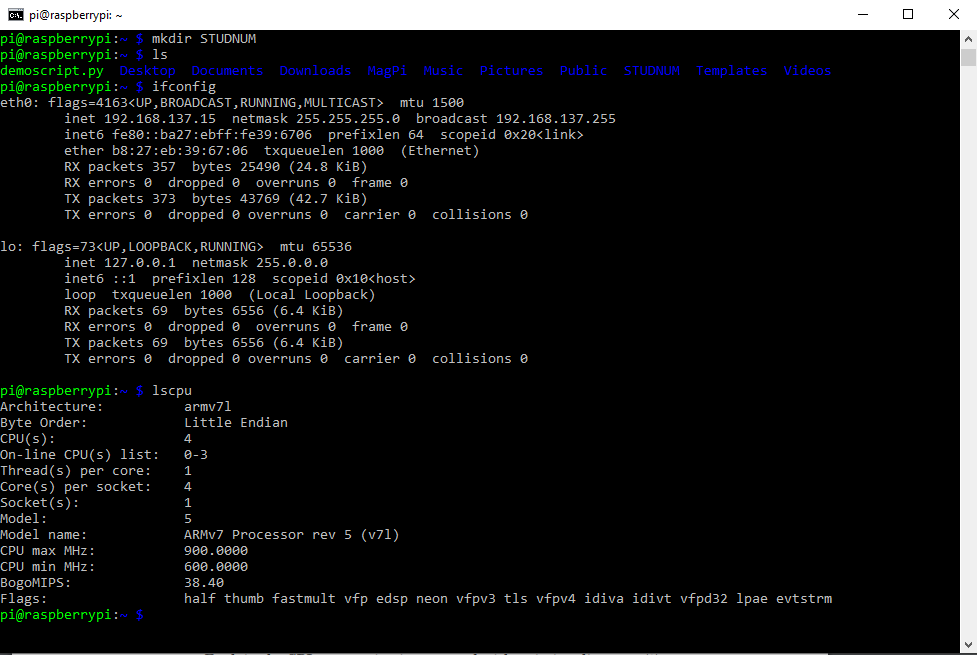
\includegraphics[width=0.6\columnwidth]{Figures/CMDOutput}
\caption{Example output after running the above commands}
\label{fig:CMDOutput}
\end{figure}



\subsubsection{Programming Task}
In this task you will develop a simple 3-bit binary counter, the values of which will be placed on LEDs connected to the Pi. The value on the counter should change depending on a button press.
Be sure to use git to keep track of changes to your code. For instructions on using Git, refer to the lab handbook.
\begin{itemize}
\itemsep0em 
    \item Start by connecting to your Pi through VNC or SSH (see lab handbook)
    \item If not installed, install the Python GPIO libraries, as explained \href{https://pythonhosted.org/RPIO/}{here}. (They should be installed by default.)
    \item Connect 3 LEDs and 2 Push buttons to the GPIO pins of the Pi - taking care of which pins to use. Look at \href{pinout.xyz}{pinout.xyz} and be sure to not use special purpose pins
    \item Read the Python Tips and tricks in the lab handbook to gain understanding of the commands and why they are used.
    \item Create a copy of the template in the mypracs folder.
    \item Write your code. It's suggested you work incrementally, committing your code using git each time you accomplish something. 
    \begin{itemize}
    \itemsep0em 
        \item Take a look at the RPI.GPIO examples, available \href{https://sourceforge.net/p/raspberry-gpio-python/wiki/Examples/}{here}
        \item Start by turning on and off a single LED in the main() method. Delay between toggling the GPIO by using something like \verb|time.sleep()|
        \item Now, use a button to toggle the state of the LED. Look at the lab handbook for help with debouncing and interrupts in Python.
        \item Finally, implement a system that displays a binary value on 3 LEDs. Use one button to increase the value, and another button to decrease the value. The values should wrap around (i.e. increasing "111" should then display "000" and decreasing "000" should display "111"
    \end{itemize}
    \item Hints
    \begin{itemize}
    \itemsep0em 
        \item Look at \textit{itertools.product} to generate a list of binary values.
        \item Use a single integer counter as an index to the Python array that you've created. Make use of Python's \verb|global| construct to do so
    \end{itemize}
    \item Demonstrate this implementation to a tutor to get signed off, and push your code to GitHub.
    \item Submit a PDF as per the deliverables section
\end{itemize}

\subsection{Mark Allocations}
Marks will be given for:
\begin{itemize}
\itemsep0em 
    \item Correctly completing the terminal task
    \item Well structured and commented code
    \item Meaningful git commit messages
    \item A correct demonstration
\end{itemize}
Marks will be deducted for:
\begin{itemize}
\itemsep0em 
    \item Not using interrupts and debouncing on your button presses
    \item Not submitting files in the correct format
    \item Not linking to the practical on GitHub
    \item Copying another student's code
    \item Late submission
\end{itemize}